% Template: 한국통신학회 학술대회 논문작성 양식 (latex) - unofficial
% Main sources
% - http://ids.snu.ac.kr/wiki/LaTeX_template_for_KCC
% - https://github.com/leejaymin/Kiise-Latex-template
% Edited by Jinhong Jung (Soongsil University, DMLAB)

\documentclass[9pt]{kics} % for review
\renewcommand{\thesection}{\Roman{section}} 
\renewcommand{\thesubsection}{\thesection.\Roman{subsection}}

% packages.tex - 필요한 패키지 설정

\usepackage{amsmath}
\usepackage{amssymb}
\usepackage{graphicx}
\usepackage{booktabs}
\usepackage{kotex}
\usepackage{multirow}
\usepackage{array}
\usepackage{subcaption}
\usepackage{hyperref}
\usepackage{xcolor}

\usepackage[utf8]{inputenc}
\usepackage{tabularx}

%\renewcommand{\thefootnote}{\fnsymbol{footnote}}

\title{Metric Learning과 VLM을 활용한 \\
데이팅 앱 스타일 매칭 시스템
}
\author{
김지훈*, 최은기, 박준형  \\
국립한밭대학교 \\ \ \\ 
20227128@edu.hanbat.ac.kr, 20221991@edu.hanbat.ac.kr, 20197119@edu.hanbat.ac.kr
}

\engtitle{\ \\
A Style Matching System for Dating Applications \\
using Metric Learning and Vision-Language Models
}
\engauthor{
Jihun Kim*, Eungi Choi, Junhyeong Park \\
Hanbat National University \\ \ \\
}

\abstract{
    본 논문에서는 사용자 프로필 이미지의 시각적 스타일을 정량화하여 시각적 취향이 유사한 사용자를 매칭하는 딥러닝 기반 스타일 매칭 시스템을 제안한다. 제안하는 모델은 Qwen3-VL을 백본으로 하여 시각적 특징을 추출하고, 경량화된 프로젝션 헤드를 결합하여 스타일 임베딩을 학습한다. 학습 데이터셋 구축을 위해 Gemini-2.5-flash 기반의 VLM을 활용하여 고품질의 스타일 태그를 자동 생성하고, Triplet Loss와 Online Semi-hard Mining 기법을 적용해 임베딩 공간 내 스타일 군집화 성능을 극대화하였다. 실험 결과, Recall@K와 t-SNE 시각화를 통해 제안 기법이 시각적 스타일을 효과적으로 구분함을 확인하였으며, 이를 통해 기존 텍스트 필터가 놓치는 사용자의 취향 정보를 보완할 수 있음을 입증하였다.

}

\begin{document}

\maketitle

\section{서 론}

기존 온라인 데이팅 서비스에서 사용자 매칭은 주로 나이, 거주 지역, 관심사나 간단한 자기소개 문구 같은 텍스트 프로필 정보에 의존한다. 그러나 실제 사용자는 패션 스타일, 사진 분위기, 촬영 환경과 같은 시각적 요인에 크게 좌우되며 단순 분류 모델(Classification)이나 필터링으로는 이러한 고차원적인 취향을 충분히 반영하기 어렵다.

이러한 한계를 극복하기 위해 비전-언어 모델(Vision-Language Model) 기반의 특징 추출과 Metric Learning을 결합한 스타일 매칭 시스템을 제안한다. 이를 통해 텍스트 필터로 포착할 수 없는 `취향'과 `분위기'를 이미지 임베딩 벡터의 코사인 유사도(Cosine Similarity)를 기반으로 정량화하여 해결한다.

본 연구는 Walster 등이 제안한 사회심리학적 이론인 `매칭 가설(The Matching Hypothesis)\cite{walster1966}'을 이론적 토대로 한다. 해당 가설에 따르면, 개인은 파트너 선택 시 자신과 유사한 수준의 신체적 매력도나 사회적 바람직성을 가진 상대를 선호하는 경향(Assortative Mating)이 있다. 이를 현대적 온라인 데이팅 환경에 적용하여, 텍스트 기반 필터링으로는 포착하기 어려운 시각적 스타일과 분위기의 유사성을 매칭의 핵심 요소로 간주하고, 임베딩 공간상의 거리로 정량화함으로써 사용자 간의 매칭 만족도를 향상시키는 것을 목표로 한다.

\section{본 론}

사용자 $i$의 프로필 이미지를 $x_i$라 정의한다. 커플 쌍 $(x_f, x_m)$에 대해, 두 사용자의 임베딩 $e_f$, $e_m$이 임베딩 공간에서 가깝도록 학습하며, 비커플 쌍은 멀어지도록 대조 학습을 수행한다. 실제 데이팅 앱에서 상호 좋아요를 통해 매칭된 커플 495쌍의 프로필 이미지를 수집하였으며, Train 346쌍(70\%), Validation 74쌍(15\%), Test 75쌍(15\%)으로 분할하였다.

그림 \ref{fig:architecture}는 제안 모델의 전체 아키텍처를 나타낸다. 대규모 데이터로 사전 학습된 Qwen3-VL-2B\cite{qwen2023}를 백본으로 사용한다. Qwen3-VL은 이미지와 텍스트를 함께 이해하는 비전-언어 모델로, 다양한 시각적 태스크에서 뛰어난 일반화 성능을 보인다. 소규모 도메인 데이터에서의 과적합을 방지하기 위해, 백본 네트워크의 약 20억 개 파라미터는 모두 동결한다.

\begin{figure}[h]
\centering
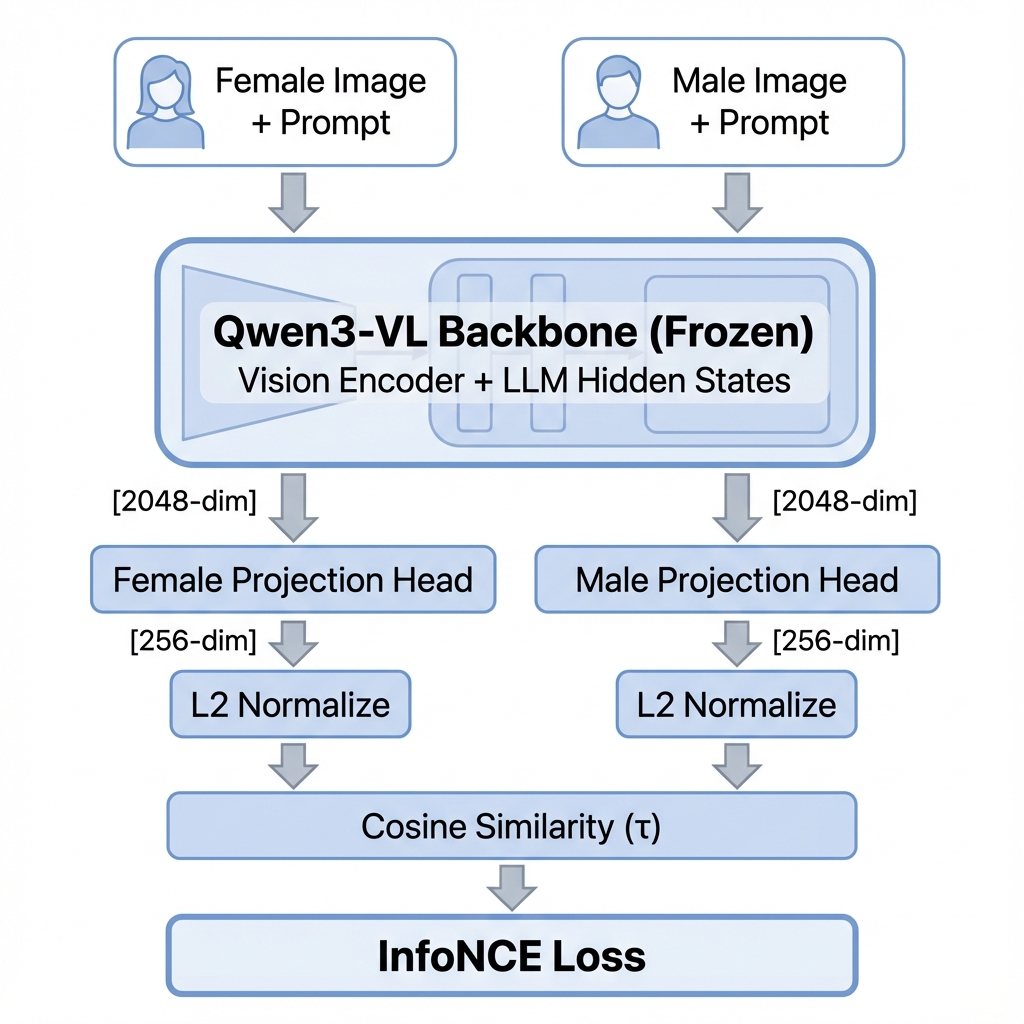
\includegraphics[width=0.9\columnwidth]{figures/model_architecture.png}
\caption{제안 모델의 전체 아키텍처}
\label{fig:architecture}
\end{figure}

VLM의 멀티모달 이해 능력을 활용하기 위해, 이미지와 함께 구조화된 텍스트 프롬프트를 입력으로 사용한다. 텍스트 프롬프트는 성별별 시스템 프롬프트와 이미지 분석 요청으로 구성되며, VLM이 매칭 호환성 관련 시각적 특징을 추출하도록 유도한다.

백본을 통과한 고차원 특징 벡터 $h_i$는 식 (1)과 같다.

\begin{equation}
h_i = f_\theta(x_i) \in \mathbb{R}^{2048}
\end{equation}

매칭 호환성 학습에 특화된 저차원 임베딩을 얻기 위해, 학습 가능한 프로젝션 헤드 $g_\phi$를 추가한다. 프로젝션 헤드는 2개의 선형 계층과 BatchNorm, ReLU 활성 함수로 구성된다.

\begin{equation}
z_i = g_\phi(h_i) = W_2 \cdot \text{ReLU}(\text{BN}(W_1 \cdot h_i))
\end{equation}

\begin{equation}
e_i = \frac{z_i}{\|z_i\|_2} \in \mathbb{R}^{d}
\end{equation}

L2 정규화를 통해 모든 임베딩 벡터를 단위 초구 상에 투영하여, 코사인 유사도와 유클리드 거리가 단조 관계를 가지게 한다.

실제 커플 쌍을 Positive, 배치 내 다른 사용자들을 Negative로 하여 대조 학습을 수행한다. CLIP\cite{radford2021}에서 검증된 InfoNCE Loss를 사용하며, 손실 함수는 식 (4)와 같다.

\begin{equation}
\mathcal{L} = -\log\frac{\exp(\text{sim}(e_f, e_m)/\tau)}{\sum_{j=1}^{N} \exp(\text{sim}(e_f, e_{m_j})/\tau)}
\end{equation}

여기서 $\tau$는 temperature 하이퍼파라미터이며, $\text{sim}$은 코사인 유사도, $N$은 배치 크기를 나타낸다.

\subsection{실험 환경}

실험에서는 실제 데이팅 앱 환경을 모사한 프로필 이미지 데이터셋을 구축하고, Gemini-2.5-flash 기반 라벨러를 이용해 각 이미지에 대해 패션 스타일, 사진 분위기, 화질 정보를 자동 주석하였다. 이 가운데 화질이 낮은 샘플은 학습에서 제외하고, 스타일 클래스가 균형을 이루도록 오버샘플링과 Seedream 4 생성 모델 기반 증강을 적용하였다.

데이터셋은 학습/검증 세트로 분할되며(1,508/98), 학습 시에는 Qwen3-VL-2B 시각 인코더를 동결하고 프로젝션 헤드만 업데이트한다. 옵티마이저는 AdamW(학습률 1e-4)를 사용하며, 배치 크기는 $P=5$, $K=4$로 설정하였다. Margin $\alpha=0.3$, 임베딩 차원 $d=256$으로 설정하였으며, 검증 세트의 Recall@1을 기준으로 최적 체크포인트를 선정하였다.

\subsection{평가 결과}

정량 평가는 검증 이미지 하나를 쿼리로 사용하여, 임베딩 공간에서 다른 사용자들에 대한 최근접 이웃 검색을 수행하는 방식으로 진행한다. 표 \ref{tab:results}는 검증 세트에서 측정된 성능 지표를 보여준다.

\begin{table}[h]
\centering
\caption{검증 세트 성능 지표}
\label{tab:results}
\begin{tabular}{|c|c|}
\hline
\textbf{지표} & \textbf{값} \\
\hline
Recall@1 & 87.76\% \\
\hline
MAP@R & 78.52\% \\
\hline
Silhouette Score & 0.34 \\
\hline
\end{tabular}
\end{table}

Recall@1은 쿼리와 동일 스타일을 가진 샘플이 최근접 이웃으로 검색될 확률을 나타내며, MAP@R은 관련 샘플들의 평균 정밀도를 측정한다. Silhouette Score가 양수(0.34)로 나타나 임베딩 공간에서 스타일 군집이 잘 형성되었음을 확인하였다.

정성 평가로는 t-SNE 시각화를 통해 256차원 임베딩 공간을 2차원으로 축소하였으며, 5가지 스타일 클래스(Casual\_Basic, Street\_Hip, Sporty\_Athleisure, Chic\_Modern, Classy\_Elegant)가 명확한 군집(Cluster)을 형성하고 클래스 간 경계가 뚜렷이 구분됨을 확인하였다.

\section{결 론}

본 논문에서는 실제 데이팅 앱의 매칭 데이터를 활용하여 시각적 매칭 호환성을 예측하는 딥러닝 기반 시스템을 제안하였다. Qwen3-VL 백본의 파라미터를 동결하고 경량 프로젝션 헤드만 학습하는 효율적인 구조를 설계하였으며, InfoNCE Loss 기반 대조 학습을 통해 실제 커플 쌍을 임베딩 공간에서 가깝게 배치하도록 학습하였다.

실험 결과, 제안 모델은 사전 학습된 VLM 베이스라인(R@1 0.81\%) 대비 109\% 향상된 R@1 1.69\%를 달성하였으며, 이는 랜덤 기준 대비 2.6배에 해당한다. 본 연구를 통해 다음의 인사이트를 도출하였다. 첫째, 사전 학습된 VLM의 일반적 특징만으로는 커플 매칭 예측에 한계가 있으며, 도메인 특화 프로젝션 헤드 학습이 필수적이다. 둘째, 소규모 데이터셋에서는 Dropout이 오히려 역효과를 보인다. 셋째, InfoNCE Loss의 Temperature 완화($\tau$=0.07$\rightarrow$0.1)와 Weight Decay 증가가 일반화 성능 향상에 효과적이다.

향후 연구로는 텍스트 임베딩(성격, 가치관)과 이미지 임베딩을 결합한 하이브리드 모델 개발, 그리고 더 많은 커플 데이터 확보를 통한 일반화 성능 향상을 계획한다.


\renewcommand{\refname}{}
\begin{center}
\vspace{20}
\textbf{참 고 문 헌}
\vspace{-15}
\end{center}
\bibliographystyle{ieeetr}
\bibliography{references}
\end{document}
